% Chapter Template

\newcommand{\reals}[1]{\mathbb{R}^{#1}}

\chapter{Proposals} % Main chapter title
\label{Chapter3}

As we have already seen in Chapter \ref{Chapter2}, LUSI introduces a new data-driven learning
paradigm which aims to find better approximations of the conditional probability function using
statistical invariants. However, these invariants are often problem dependent and choosing the
appropriate ones is not an easy task, as there are many possible ones and some of them are not
straightforward to come up with.

Thus, our main goal with this work is to create a series of new invariants which we expect to be of
general use, as well as automatizing the selection process of the invariants that should be considered
for a given problem and extending the LUSI paradigm to multiclass problems\footnote{Even though in the
original paper the authors state that the method can be applied to multiclass problems, they do not go
into too much detail of how this is done.}.

In this chapter we are going to present our proposals, which are a two new invariants based on randomness
which aim to be more general than the original ones and an extension of the LUSI paradigm to multiclass problems
using Error Correcting Output Codes (ECOC).

\section{Random invariants}

Our first proposal is a series of random invariants, which are invariants that have some sort of random
process inside of them but that aim to preserve some sort of statistical information of the data. This way,
we aim to greatly reduce the amount of necessary prior knowledge of the problem when choosing which invariants
to use, treating it just like any other hyperparameter of a machine learning model. In this work, we propose
an invariant based on random projections as well as another one based on random hyperplanes.

\subsection{Random projections}

Random projections have been frequently used in the machine learning field to perform dimensionality reduction
in a faster and computationally less expensive way than other techniques (i.e., PCA) as studied in 
\cite{Dasgupta2000} and \cite{BinghamManila2001}.

In this case, the random projection invariant projects the data into a new one-dimensional space,
as if it was viewed from a particular point in the original space. In some way, it is like having
different compressed views of the same data. Intuitively, this can be observed in figure
\ref{fig:random_projections_example}.

More formally speaking, consider a data point $x \in \reals{d}$ and a projection vector
$p \sim \mathcal{N}(\mu, \Sigma)$, where the multivariate normal distribution has mean $\mu \in \reals{d}$
and covariance matrix $\Sigma \in \reals{d \times d}$. We can define the random projection invariant as follows:

\begin{equation}
    \label{eq:random_projection_invariant}
    \psi_{r.p.}(x) = x p
\end{equation}

As we can see in expression \eqref{eq:random_projection_invariant}, we are computing the dot product between
the data point and the projection vector. When this invariant is used in expression \ref{eq:invariant_approximation}
it will try to preserve the centroid of the positive class in the new projected space. Hence, it is a variation
of the first order invariant. When using multiple random projections as invariants, we expect that the centroid
of the positive class is preserved across different views of the data.

\begin{figure}[h]
    \centering
    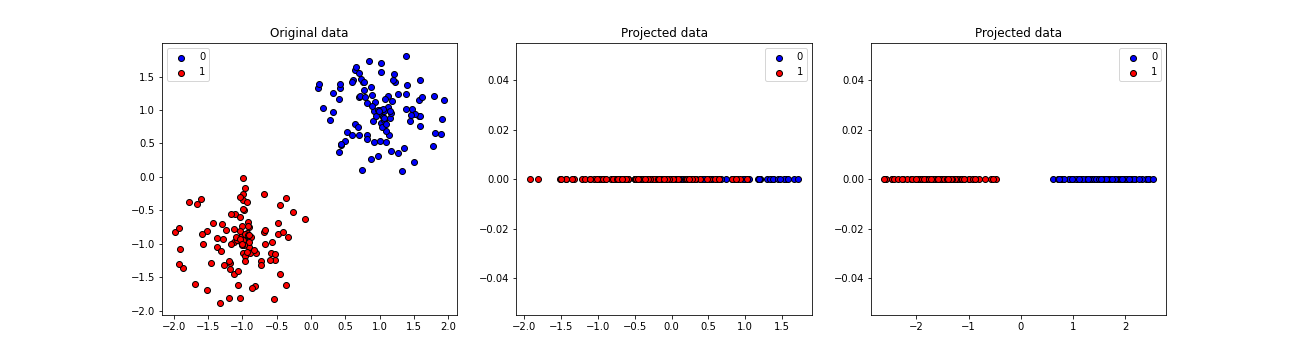
\includegraphics[width=\textwidth]{thesis/Figures/random_projections_example}
    \caption{Example of a dataset and two random projections of it. In the first projection, we can see
    that the points from the positive and the negative classes are almost totally overlapped, whereas in the
    second projection they are completely separable.}
    \label{fig:random_projections_example}
\end{figure}

\subsection{Random hyperplanes}

The second invariant that we propose is the random hyperplane. With it, we aim to create two partitions of
the original data: the samples that are on the right side of the hyperplane and the ones on the left, which
we will consider as the positive and the negative samples, respectively. Opposite to the previous invariant, which
produced a real value when applied to a point $x$, this one produces a discrete value $\set{0, 1}$ based on the
relative position of the point with respect to the normal vector of the hyperplane.
Figure \ref{fig:random_hyperplanes_example} shows an example of how this invariant works when applied to
an example dataset.

Formalizing the previous explanation, consider an arbitrary point from the sample $x_c \in \reals{d}$. Let
$n \sim \mathcal{N}(\mu, \Sigma)$ be the normal vector of the hyperplane that contains $x_c$, where the
multivariate normal distribution has mean $\mu \in \reals{d}$ and covariance matrix $\Sigma \in \reals{d \times d}$.
We can define the random hyperplane invariant as

\begin{equation}
    \label{eq:random_hyperplane_invariant}
    \psi_{r.h.}(x) =
    \begin{cases}
        1 & \text{if $(x - x_c)n \geq 0$ }\\
        0 & \text{otherwise}
    \end{cases}
\end{equation}

Considering the previous expression, we can clearly see that this invariant will yield a vector of zeroes
and ones when applied to a dataset. If we also take into account expression \eqref{eq:invariant_approximation},
we can deduce that this invariant will try to preserve the proportion of positive samples that fall on the right
side of the hyperplane. Consequently, we can see that this is a variation of the zeroth order invariant.
The main difference is that we are now trying to preserve the proportion of positive elements in a subspace
of the original space (the subspace formed by the samples that are on the same side as the normal vector of the
hyperplane), instead of trying to preserve it in the whole space.

\begin{figure}[h]
    \centering
    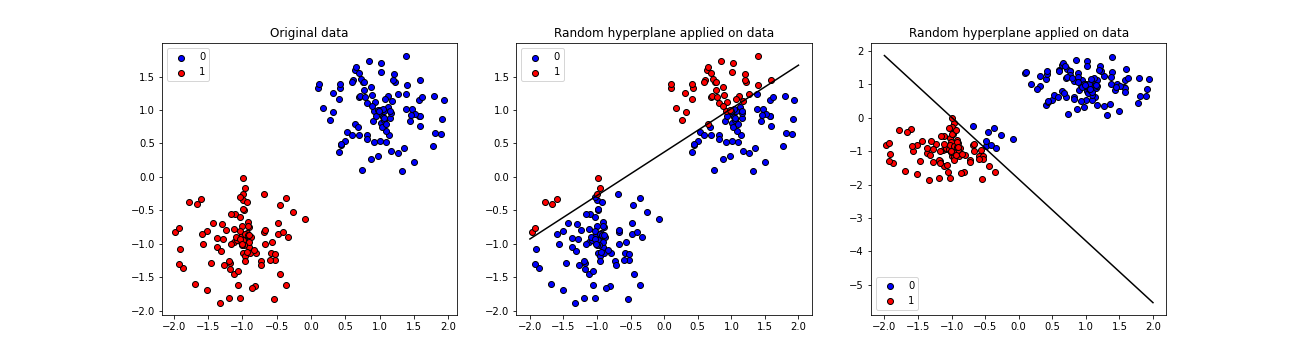
\includegraphics[width=\textwidth]{thesis/Figures/random_hyperplanes_example.png}
    \caption{Example of the hyperplanes invariant. In the left image, we can see the original data. In
    the middle and right images we can see two hyperplanes that divide the data in elements which are
    on the right and the left of the hyperplane, labeled as 1 and 0 respectively. Note that these
    new labels do not necessarily match the original ones.}
    \label{fig:random_hyperplanes_example}
\end{figure}

\section{Extending the LUSI paradigm to multiclass problems}

As we have seen up until now, this learning paradigm can be easily applied to binary classification problems
and solve them. Nevertheless, note that the invariants are defined specifically for just one of the classes. This ignores the invariant information that could be gathered by considering the other class. Moreover, in the most general setting of multiclass classification, the algorithm has to be extended. So, instead of restraining ourselves to a particular kind of problems, it seems reasonable trying to extend
LUSI to multiclass problems so that we have a wider application scope.

One framework that can be used to easily deal with this kind of problems is Error Correcting Output Codes (ECOC),
introduced by \cite{DietrichBakiri1995}. We can use it to treat multiclass classification problems as if they
were binary. For each one of the $N_c$ classes we create a codeword of length $n$. These codewords can be arranged as
the rows of a matrix called the \emph{coding matrix} $M \in \set{0, 1}^{N_c \times n}$. Each column of the matrix
is treated as an individual binary classification problem and a binary classifier is trained for each one of these
problems using the corresponding encoding (the columns).

An example of this can be seen in tables \ref{tab:ecoc_example_identity} and \ref{tab:ecoc_example_complex},
which show two different coding matrices for the same 5-class classification problem. The first one encodes the
problem as five one-against-all problems, which means that in each problem there will be only one class that can be
considered the positive one. In the second matrix, we can appreciate that some classes are encoded more than
once as the positive class.

\begin{table}[H]
\centering
\begin{tabular}{c|ccccc}
            & $h_1$ & $h_2$ & $h_3$ & $h_4$ & $h_5$ \\ \hline
\textbf{C1} & 1     & 0     & 0     & 0     & 0     \\
\textbf{C2} & 0     & 1     & 0     & 0     & 0     \\
\textbf{C3} & 0     & 0     & 1     & 0     & 0     \\
\textbf{C4} & 0     & 0     & 0     & 1     & 0     \\
\textbf{C5} & 0     & 0     & 0     & 0     & 1    
\end{tabular}%
\caption{Coding matrix for a multiclass classification problem with 5 classes and codewords of length $n=5$.
This matrix defines a special coding called one-against-all.}
\label{tab:ecoc_example_identity}
\end{table}


\begin{table}[H]
\centering
\begin{tabular}{c|ccccc}
            & $h_1$ & $h_2$ & $h_3$ & $h_4$ & $h_5$ \\ \hline
\textbf{C1} & 1     & 1     & 1     & 0     & 0     \\
\textbf{C2} & 0     & 1     & 1     & 0     & 1     \\
\textbf{C3} & 1     & 0     & 0     & 1     & 0     \\
\textbf{C4} & 0     & 1     & 0     & 1     & 0     \\
\textbf{C5} & 0     & 0     & 1     & 0     & 1    
\end{tabular}
\caption{Another coding matrix for the same 5-class classification problem.}
\label{tab:ecoc_example_complex}
\end{table}

Suppose that we have already trained a binary classifier for each one of the problems and we want to
predict the class for a given data point $x$. Let us denote $f(x) = (f_1(x), \dots, f_n(x))$ the
vector containing the predictions for each one of the problems. In order to obtain the corresponding output
class, we would need to decode this vector of predictions using the coding matrix that we have defined
for the problem. This is usually done by using some kind of distance metric and selecting the class with
the closest codeword according to the selected metric.

There are many distance metrics that we could use: Hamming distance, Euclidean distance, etc. In this
particular case, we have considered the Euclidean distance, which we will denote as $d_E$ and is computed
as $d_e(x, x') = \norm{x - x'}_2$. Let $M_r \in M$ be the $r$-th row of the coding matrix
We can express the predicted class $\hat{y}$ as

\begin{equation}
    \label{eq:ecoc_decoding}
    \hat{y} = \argmin_r d_E(M_r, f(x))
\end{equation}

Thus, the predicted class will be the one associated to the row that is closest to the vector of predictions.
Something important that we have to consider is that the binary classifiers for each problem should return the
probability $P(y=1 | x)$ rather than the actual label, which means that no threshold should be applied
during the prediction stage. This is because using the label directly might cause some errors when computing
the closest codeword. For example, consider the coding matrix defined in \ref{tab:ecoc_example_identity} and that
we are given a vector of predictions $(1, 1, 0, 0, 0)$ whose associated vector of probabilities is
$(0.8, 0.55, 0.4, 0.1, 0.25)$. If we consider the binary vector of predictions, then both class 1 and
class 2 are the closest ones, which will lead to randomly selecting among them and to a potential missclassification
since class 1 is the most probable 1. However, if we consider the vector of probabilities, then the closest
class in this case will be class 1, which is indeed the most probable one.

In consequence, in order to extend LUSI to multiclass classification problems we have to follow these steps:

\begin{enumerate}[label=\textbf{Step \arabic*:}]
    \item Create the coding matrix $M$ of size $N_c \times n$.
    \item Use the columns of $M$ to generate new binary labels for each one of the $n$ binary classification problems.
    \item Train $n$ binary classifiers that use LUSI with the previously generated binary labels.
    \item Given an input data point $x$, predict the vector of probabilities using the previous binary classifiers.
    \item Select the output class using expression \eqref{eq:ecoc_decoding}.
\end{enumerate}
